\documentclass[english,10pt,twocolumn]{article}

\usepackage{times}
\usepackage{fullpage}
\usepackage{babel}
\usepackage{graphicx}


\begin{document}

\title{Unikernel Web Infrastucture}
\author{Nate Brennand, Gudbergur Erlendsson, Mishail Tupas}
\date{}
\maketitle
\thispagestyle{empty}

\begin{abstract}
Traditional web infrastructure models consist of a cluster of heavyweight full stack virtual machines usually running a variant of Linux.
This provides a simple consistent platform to develop against but it has many downfalls in the resource overhead of running virtual machines.
Key-value datastores are a common component of web insfrastructure.
We've designed a Mirage OS\cite{mirage} unikernel implementation of the popular Redis\cite{redis} key-value store that allows fast creation and deployment of the datastore as well as ease scaling up the allocated resources.
We describe the advantages and disadvantages that come with such a system.
We highlight the performance characteristics of this new approach in comparison to Redis.
\end{abstract}

\section{Introduction}
In-memory key-value datastores are used in a wide variety of applications for ease of use and the high throughput.
While these applications are known for their great performance, research has shown that networked applications striving for low latency, such as Redis, are actually subjected to a high amount of overhead from utilizing Linux's networking stack.\cite{arrakis}
This issue is amplified by the lack of stability when running on Linux itself which is prone to performance dips when the resource scheduler is not coordinated.

We believe that the approach of moving the key-value datastore to a unikernel implementation will yield greater and more reliable performance.
A unikernel is a specialzed application capable of running directly on top of bare-metal or a hypervisor without a host operating system.
The unikernel approach lacks many of the performance issues plaguing Redis that cannot be resolved at the application level.
We build on top of the Mirage OS\cite{mirage}, an OCaml based library operating system that provides type-safe networking libraries.

We measure the performance characteristics of Redis in multiple situations, networked and on-host, to yield a direct comparison to our implementation, Kayvee.
Kayvee speaks the Redis Serialization Protocol\cite{redis-protocol}, RESP, which makes Kayvee a drop in replacement for Redis in any deployment utilizing the Xen Hypervisor.


\section{Background}
% unikernel backgorund
The unikernel concept was first outlined X.

Today there are server operating systems developed for cloud computing that based on the concept of unikernels. Mirage OS is a library operating system written in Ocaml that is commonly used for constructing unikernels.

% key-value datastore background
(What are key-value stores for?) 

Redis, short for Remote Dictionary server, is a key-value store software that is commonly used in distributed systems on virtualized operating systems. It features (). However, this software is generally run atop a full operating system installation, which incurs a certain degree of overhead as discussed previously.  While the OSv operating system can support Redis, it does not function optimally.

\section{Design and Implementation}

The Mirage OS unikernel library operating system is leveraged to provide a correct and compact implementation. Mirage OS leverages the Ocaml language to provide type safety at a low level, this creates many guarantees in terms of correctness.
GET Operation
SET Operation
Evaluation

To test the unikernel implementation, we utilized two of the benchmarking tools provided by the  ocam development kit. To get execution counts, the profiler “ocamlprof”, a part of the ocaml toolchain was used, inserting relevant information as comments to the code. To get detailed execution time information, the unikernel was compiled to include profiling information for the gprof tool.

Redis’ benchmarking tool was used to get data for comparison, running on both as a host system and a virtual machine. The Redis benchmarking tool was limited to four tests: inline ping, bulk ping, get method, and set method. For all tests, the benchmark made one million requests across fifty simulated parallel clients using a payload of three bytes.

The main point of comparison is the relative runtime of the unikernel implementation versus the two Redis setups. For each of the methods that were implemented
Collected Results

So far, the only benchmarks that have been completed were the Redis benchmarks for both the host-to-host setup and the native host setup. Preliminary benchmarks for the unikernel have been run.

SET Operation




\section{Evaluation}

We performed all of our evaulations on a dedicated 8\-core HP ProLiant rack server with 16 GB RAM available.
Our Xen hypervisor installation is coordinated by a Ubuntu Server 14.04 host that serves as the management domain to manage the other hosts running on the Hypervisor.
The Mirage installation was modified to use Redis' communication protocols so that we could use the same benchmark for all test setups. The benchmark was run using 50 parallel clients sending a 3-byte payload. 
The Redis setups were given ten thousands requests as part of their benchmark, while the Mirage setups on Xen were given five hundred, one thousand, or ten thousand requests.


\subsection{Running Mirage}

When a Mirage OS unikernel is configured in Xen mode, both the unikernel image and the configuration file are generated.
With these, a unikernel can be easily launched using the xl Xen management tool.
Due to the small size of the image, this is a quick process where the Mirage image configures itself when started by xl.

\subsection{Network Overhead}

On examining the throughput and the completion times for requests between running the benchmark between two hosts, we found that there was a significant overhead imposed by network communications. For SET operations there was an increase of 42\% in execution time and GET operations saw a similar 43\% increase in execution time.
The benchmark results for the Mirage OS installation were found to have throughputs an order of magnitude lower than expected. 
Upon further testing and examination of code, it found that that the Mirage systems were not properly handling multiple simultaneous clients, resulting in a very low throughput which was noticed in further tests.


\subsection{Mirage \- UNIX}

Three different benchmarks setups were tested, making either five hundred, one thousand, or ten thousand total requests. 
Similarly to the tests run on the Mirage installations that were on top of Xen, the throughput was also an order of magnitude lower when compared to Redis. 
Strangely, the Unix-based setups did much better for the five hundred and one thousand request trials, but did extremely poorly for the ten thousand request setup.

\subsection{Throughput Performance}

\begin{figure*}[ht]
  \centering
  \caption{Average Throughputs}
  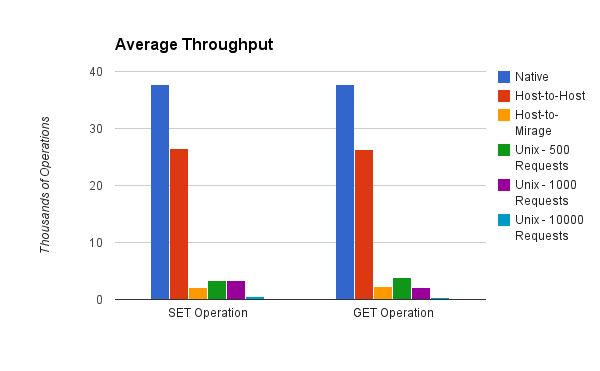
\includegraphics[width=1.0\textwidth]{images/throughput}
\end{figure*}

\begin{table}[h]
\begin{tabular}{lll}
Average Throughput & SET Operation & GET Operation \\
Native & 37766.142 & 37792.576 \\
Host-to-Host & 26571.512 & 26348.028 \\
Mirage on Xen & 2188.18 & 2222.22 \\
Unix (500) & 3401.36 & 3787.88 \\
Unix (1000) & 3344.48 & 2024.29 \\
Unix (10000) & 580.55 & 338.26
\end{tabular}
\caption{Average throughputs (requests per second)}
\label{my-label}
\end{table}

Overall, the Mirage systems showed markedly worse throughput performance, at a staggering order of magnitude lower than the baseline Redis benchmarks. 
Corrections to the Mirage coding are underway so that a fair benchmark comparison can be made and a provide a more representative view.

\section{Conclusion}
% @NATE


\section{Acknowledgements}
We thank the kind souls in the \#Mirage IRC chatroom for their relentless patience.
Their assistance was crucial in learning how to use Mirage's utilities and leverage the provided standard library.




\bibliographystyle{abbrv}
\bibliography{bibliography}


\end{document}



